% Figura: lazo PiL como diagrama de bloques de control (MARLUP, Actividad 3)
% Compilar este archivo solo:  pdflatex arquitectura_pil.tex  -> arquitectura_pil.pdf
% En el reporte:  \includegraphics[width=\columnwidth]{figuras/arquitectura_pil.pdf}
% Refleja la implementacion real (pil_ctrl.m + pil_arduino.ino):
%  - el modelo del sensor (sesgo, histeresis, ADC 10 bits) y la referencia estan en Simulink;
%  - la trama 0xAA lleva x medida y x_ref en unidades de 0.01 mm; el MCU las escala a metros;
%  - el MCU devuelve u (int16, u*32767) en la trama 0x55; en el PiL no se genera PWM;
%  - lockstep: Simulink espera u[k] antes de avanzar, la latencia de la UART no llega a la planta.
\documentclass[tikz,border=3pt]{standalone}
\usepackage[utf8]{inputenc}
\usepackage[T1]{fontenc}
\usepackage{amsmath,amssymb}
\usetikzlibrary{positioning,arrows.meta,fit,backgrounds,calc}

% Paleta (Okabe-Ito: apta para daltonismo y legible en escala de grises)
\definecolor{azulPC}{HTML}{0072B2}     % lado PC / Simulink
\definecolor{naranjaMCU}{HTML}{B36B00} % lado MCU
\definecolor{ambar}{HTML}{E69F00}      % acento: controlador
\definecolor{bermellon}{HTML}{D55E00}  % enlace serial
\definecolor{tinta}{HTML}{333333}      % texto y flechas

\begin{document}
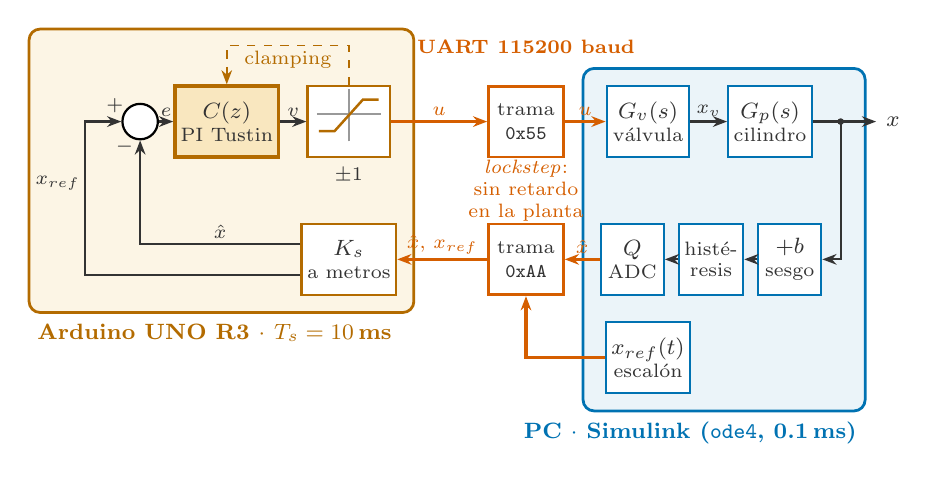
\begin{tikzpicture}[
  font=\footnotesize, text=tinta,
  >={Stealth[length=1.8mm]},
  bloque/.style={draw, line width=0.8pt, fill=white, align=center,
                 minimum width=1.05cm, minimum height=0.9cm, inner sep=2pt},
  bMCU/.style={bloque, draw=naranjaMCU},
  bPC/.style={bloque, draw=azulPC},
  bCtrl/.style={bloque, draw=naranjaMCU, line width=1.3pt, fill=ambar!25},
  bSer/.style={bloque, draw=bermellon, line width=1pt, minimum width=0.95cm},
  suma/.style={draw, circle, line width=0.8pt, fill=white, minimum size=4.5mm, inner sep=0pt},
  senal/.style={->, line width=0.8pt, draw=tinta},
  serial/.style={->, line width=1.1pt, draw=bermellon},
  nombre/.style={font=\scriptsize},
  etq/.style={font=\scriptsize, above, inner sep=1.5pt},
  contenedor/.style={rounded corners=4pt, inner sep=6pt, line width=1pt}
]

% ---------------- Coordenadas de las filas ----------------
\def\yF{0}      % camino directo
\def\yR{-1.75}  % realimentación

% ---------------- MCU: escalado, comparación, PI y saturación ----------------
\node[suma] (sum) at (0.7,\yF) {};
\node[font=\scriptsize] at ($(sum)+(-0.32,0.2)$) {$+$};
\node[font=\scriptsize] at ($(sum)+(-0.2,-0.32)$) {$-$};

\node[bCtrl] (C) at (1.8,\yF) {$C(z)$\\[-1pt]\scriptsize PI Tustin};

\node[bMCU, path picture={
      \draw[tinta!50] ($(path picture bounding box.west)+(0.12,0.1)$) -- ($(path picture bounding box.east)+(-0.12,0.1)$);
      \draw[tinta!50] ($(path picture bounding box.center)+(0,-0.25)$) -- ($(path picture bounding box.center)+(0,0.42)$);
      \draw[line width=0.9pt] ($(path picture bounding box.center)+(-0.38,-0.12)$) -- ++(0.2,0)
            -- ++(0.36,0.4) -- ++(0.2,0);}] (sat) at (3.35,\yF) {};
\node[nombre, below=0pt of sat] {$\pm1$};

% anti-windup por clamping: la saturación congela la integral
\coordinate (cl) at ($(sat.north)+(0,0.5)$);
\coordinate (izq) at (-0.5,\yF);   % margen izquierdo del MCU para la etiqueta de x_ref
\draw[->, line width=0.6pt, dashed, draw=naranjaMCU]
  (sat.north) -- (cl) -| node[pos=0.25, below, font=\scriptsize, text=naranjaMCU, inner sep=1.5pt]{clamping} (C.north);

\node[bMCU] (esc) at (3.35,\yR) {$K_s$\\[-1pt]\scriptsize a metros};

% ---------------- Enlace serial (tramas de 6 bytes) ----------------
\node[bSer] (serF) at (5.6,\yF) {\scriptsize trama\\[-1pt]\scriptsize \texttt{0x55}};
\node[bSer] (serR) at (5.6,\yR) {\scriptsize trama\\[-1pt]\scriptsize \texttt{0xAA}};

% ---------------- PC: válvula, cilindro, sensor y referencia ----------------
\node[bPC] (act) at (7.15,\yF) {$G_v(s)$\\[-1pt]\scriptsize válvula};
\node[bPC] (plt) at (8.7,\yF) {$G_p(s)$\\[-1pt]\scriptsize cilindro};
% modelo del sensor: sesgo -> histéresis -> ADC (de derecha a izquierda)
\node[bPC, minimum width=0.8cm] (ses) at (8.95,\yR) {$+b$\\[-1pt]\scriptsize sesgo};
\node[bPC, minimum width=0.8cm] (his) at (7.95,\yR) {\scriptsize histé-\\[-2pt]\scriptsize resis};
\node[bPC, minimum width=0.8cm] (adc) at (6.95,\yR) {$Q$\\[-1pt]\scriptsize ADC};
\node[bPC] (ref) at (7.15,{\yR-1.25}) {$x_{ref}(t)$\\[-1pt]\scriptsize escalón};

\coordinate (brk) at ($(plt.east)+(0.45,0)$);

% ---------------- Contenedores ----------------
\begin{scope}[on background layer]
  \node[contenedor, draw=naranjaMCU, fill=ambar!10, fit=(izq)(sum)(C)(sat)(esc)(cl),
        label={[font=\footnotesize\bfseries, text=naranjaMCU, anchor=north west]south west:Arduino UNO R3 $\cdot$ $T_s=10$\,ms}] (mcu) {};
  \node[contenedor, draw=azulPC, fill=azulPC!8, fit=(act)(plt)(ses)(his)(adc)(ref)(brk),
        label={[font=\footnotesize\bfseries, text=azulPC, anchor=north east]south east:PC $\cdot$ Simulink (\texttt{ode4}, 0.1\,ms)}] (pc) {};
\end{scope}

% ---------------- Camino directo ----------------
\draw[senal] (sum) -- node[etq]{$e$} (C);
\draw[senal] (C) -- node[etq]{$v$} (sat);
\draw[serial] (sat) -- node[etq, text=bermellon]{$u$} (serF);
\draw[serial] (serF) -- node[etq, text=bermellon]{$u$} (act);
\draw[senal] (act) -- node[etq]{$x_v$} (plt);
\draw[senal] (plt.east) -- ++(0.8,0) coordinate (salida) node[right]{$x$};

% ---------------- Realimentación ----------------
\fill[tinta] ($(plt.east)+(0.35,0)$) circle (1.2pt);
\draw[senal] ($(plt.east)+(0.35,0)$) |- (ses.east);
\draw[senal] (ses) -- (his);
\draw[senal] (his) -- (adc);
\draw[serial] (adc) -- node[etq, text=bermellon]{$\hat{x}$} (serR);
\draw[serial] (ref.west) -| (serR.south);
\draw[serial] (serR) -- node[etq, text=bermellon]{$\hat{x},\,x_{ref}$} (esc);
\draw[senal] ($(esc.west)+(0,0.2)$) -| node[pos=0.25, etq]{$\hat{x}$} (sum.south);
\draw[senal] ($(esc.west)+(0,-0.2)$) -- (0.0,{\yR-0.2}) |- node[pos=0.3, left, font=\scriptsize, inner sep=1.5pt]{$x_{ref}$} (sum.west);

% ---------------- Anotaciones del enlace ----------------
\node[font=\scriptsize\bfseries, text=bermellon] at (5.6,0.95) {UART 115200 baud};
\node[font=\scriptsize, text=bermellon, align=center] at (5.6,{\yR/2})
     {\textit{lockstep}:\\sin retardo\\en la planta};

\end{tikzpicture}
\end{document}
